\documentclass[a4paper,11pt]{article} 

\usepackage[english]{babel}
\usepackage[utf8]{inputenc}
\usepackage{amsmath,amssymb}
\usepackage{graphicx}
\usepackage{tikz}
\usetikzlibrary{shapes}
\usepackage{natbib}
\usepackage{hyperref}

\title{Testing HTML Export with make4ht}

\author{LianTze Lim}

\date{}

\begin{document}
\maketitle

\begin{abstract}
Your abstract. Ça va? (Yes accented characters work.)
\end{abstract}

\section{Overview of Steps}

\begin{equation}
MAE_t = \frac{1}{min(n',t)} \sum_{i=max(t-n'+1,1)}^{t}  \| \hat{y}_i - y_i \|; 
\end{equation}

\begin{equation}
S(\omega)=1.466\, H_s^2 \frac{\omega_0^5}{\omega^6} \exp\Bigl[-3^{\frac{\omega}{\omega_0}}\Bigr]^2
    \end{equation}
    
\begin{equation}
S(\omega)=1.466\, H_s^2 \,  \frac{\omega_0^5}{\omega^6}  \, e^{\left[-3^{\omega/(\omega_0)}\right]^2}
\end{equation}    
    
    
\begin{equation}SA = Round\left( \left[1 - \frac{MAE(App)}{MAE(Median)}\right]*100 \right),
\end{equation}




\begin{enumerate}
\item I tweaked the \verb|latexmkrc| file so that \verb|make4ht| is run along with \verb|pdflatex|, so the HTML export is done only if you set your project to be compiled with \verb|pdflatex|.

(\verb|make4ht| doesn't work well with \verb|fontspec|; I haven't time to try this workflow with \verb|XeLaTeX| nor \verb|LuaLaTeX| yet. So let's just leave it at \verb|pdflatex| first, yeah?)

\item \verb|my.cfg| contains the settings I usually use in my workflow:
  \begin{itemize}
  \item Output math as MathML, and render it in browsers using MathJax.
  \item When \verb|\includegraphics| uses \verb|.jpg|, \verb|.png|, \verb|.jpg|, \verb|.svg|, use the files directly for the HTML without conversion.
  \item When \verb|\includegraphics| uses \verb|.eps| and \verb|.pdf|, convert them to \verb|.png| using ImageMagick \verb|convert|, and use those for the HTML.

  \item Tikz drawings are output as \verb|.svg|.
  
  \item I've included some CSS styling. You can add a separate \verb|.css| file for further styling.
  \end{itemize}
  
\item When compilation is complete, use the steps at \href{https://www.overleaf.com/learn/how-to/View_generated_files}{\emph{View generated files}} to download each generated file required. There's also a \texttt{allfiles.zip} that contains \emph{all} generated files.
\end{enumerate}

\subsection{Caveats}

\begin{itemize}
\item This is an experimental hackety hack -- things may just not work! More a proof-of-concept rather than a stable solution on Overleaf at present.
\item tex4ht doesn't work well with \verb|fontspec| nor \verb|authblk|.
\item Avoid \verb|\mathbf| -- this broke MathML and MathJax for me.
\item Avoid, or re-define the \verb|multicol| environment to do nothing -- tex4ht will really export text in two or three columns \emph{by PDF page}, and it's not the most readable.
\end{itemize}

\section{Introduction}

Your introduction goes here! 

\section{Some \LaTeX{} Examples}
\label{sec:examples}

\subsection{How to Include Figures}

First you have to upload the image file (JPEG, PNG or PDF) from your computer to writeLaTeX using the upload link the project menu. Then use the includegraphics command to include it in your document. Use the figure environment and the caption command to add a number and a caption to your figure. See the code for Figure \ref{fig:frog} in this section for an example.

\begin{figure}
\centering
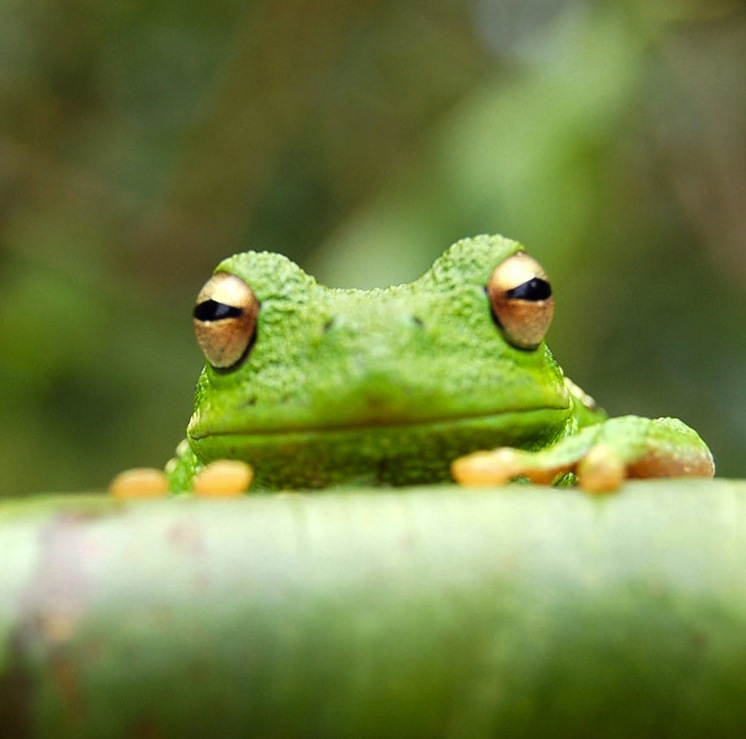
\includegraphics[width=0.3\textwidth]{frog}
\caption{\label{fig:frog}This frog was uploaded to Overleaf via the project menu. The \texttt{.jpg} file will be used as-is in the HTML export.}
\end{figure}

\begin{figure}
\centering
\includegraphics[width=0.3\textwidth]{overleaf}
\caption{PDF images will be converted to PNG when exported to HTML.}
\end{figure}

\subsection{How to Make Tables}

Use the table and tabular commands for basic tables --- see Table~\ref{tab:widgets}, for example.

\begin{table}
\centering
\begin{tabular}{l|r}
Item & Quantity \\\hline
Widgets & 42 \\
Gadgets & 13
\end{tabular}
\caption{\label{tab:widgets}An example table.}
\end{table}

\subsection{How to Write Mathematics}

\LaTeX{} is great at typesetting mathematics. Let $X_1, X_2, \ldots, X_n$ be a sequence of independent and identically distributed random variables with $\text{E}[X_i] = \mu$ and $\text{Var}[X_i] = \sigma^2 < \infty$, and let
$$S_n = \frac{X_1 + X_2 + \cdots + X_n}{n}
      = \frac{1}{n}\sum_{i}^{n} X_i$$
denote their mean. Then as $n$ approaches infinity, the random variables $\sqrt{n}(S_n - \mu)$ converge in distribution to a normal $\mathcal{N}(0, \sigma^2)$.

In this HTML export example, math is output as MathML, and will be rendered using MathJax.

\subsection{How to Make Sections and Subsections}

Use section and subsection commands to organize your document. \LaTeX{} handles all the formatting and numbering automatically. Use ref and label commands for cross-references.

\subsection{How to Make Lists}

You can make lists with automatic numbering \dots

\begin{enumerate}
\item Like this,
\item and like this.
\end{enumerate}
\dots or bullet points \dots
\begin{itemize}
\item Like this,
\item and like this.
\end{itemize}
\dots or with words and descriptions \dots
\begin{description}
\item[Word] Definition
\item[Concept] Explanation
\item[Idea] Text
\end{description}

Testing some citations: \cite{NTLKProject2015,Bond2014}

\section{Tikz Drawings}

TikZ drawings will be output as SVG, which should be rendered by most modern browsers.

\begin{figure}
\centering
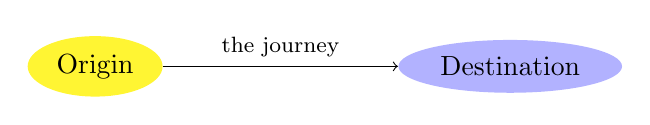
\begin{tikzpicture}
\node[fill=yellow!80,ellipse] (origin) {Origin};
\node[fill=blue!30,ellipse] (destination) at (15em,0) {Destination};
\path (origin) edge[->] node[above,font=\footnotesize] {the journey} (destination);
\end{tikzpicture}
\caption{TikZ drawings will be output as SVG, which should be rendered by most modern browsers.}
\end{figure}

\bibliographystyle{unsrt}
\bibliography{references}

\end{document}